\chapter*{\textbf{Эксперимент №1: Исследования расслоения динамической памяти}}
\addcontentsline{toc}{chapter}{Эксперимент №1: Исследования расслоения динамической памяти}

\subsection*{\textbf{Цель эксперимента}}
Определение способа трансляции физического адреса, используемого при обращении к динамической памяти. 

\subsection*{\textbf{Описание проблемы}}
В связи с конструктивной неоднородностью оперативной памяти, обращение к последовательно расположенным данным требует различного времени.
В связи с этим, для создания эффективных программ необходимо учитывать расслоение памяти, характеризуемое способом трансляции физического адреса.

\subsection*{\textbf{Исходные данные}}
Размер линейки кэш-памяти верхнего уровня; объем физической памяти.

\subsection*{\textbf{Результаты эксперимента}}
На рисунке \ref{img:experiment_1_1} представлен график, полученный в результате эксперимента с исходными параметрами:
\begin{itemize}
	\item максимальное расстояния между	читаемыми блоками (К) = 128;
	\item шаг увеличения расстояния между читаемыми 4-х байтовыми ячейками (Б) = 128;
	\item размер массива (М) = 1.
\end{itemize}

\begin{figure}[H]
	\centering{
		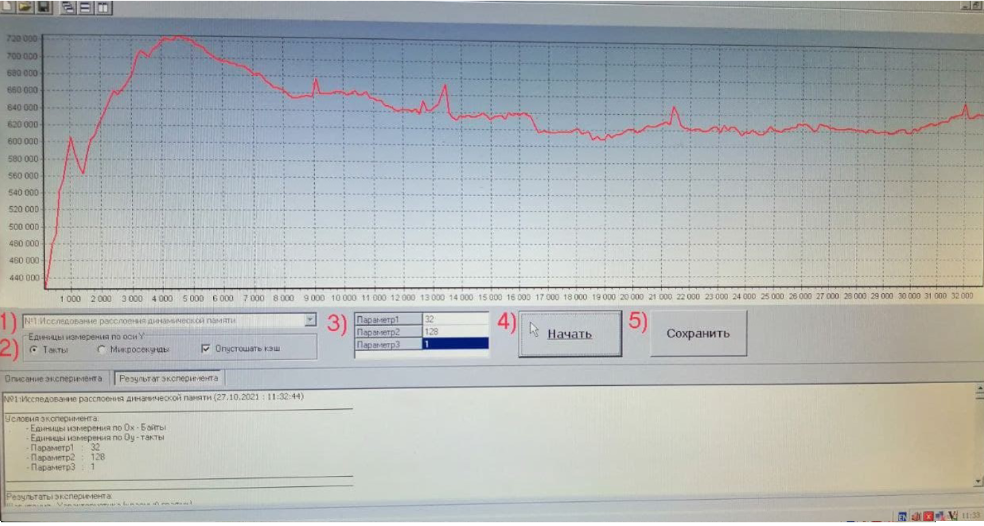
\includegraphics[scale=0.7]{images/experiment_1_1}
		\caption{Эксперимент №1,случай 1}
		\label{img:experiment_1_1}
	}
\end{figure}

На рисунке \ref{img:experiment_1_2} представлен график, полученный в результате эксперимента с исходными параметрами:
\begin{itemize}
	\item максимальное расстояния между	читаемыми блоками (К) = 128;
	\item шаг увеличения расстояния между читаемыми 4-х байтовыми ячейками (Б) = 32;
	\item размер массива (М) = 1.
\end{itemize}

\begin{figure}[H]
	\centering{
		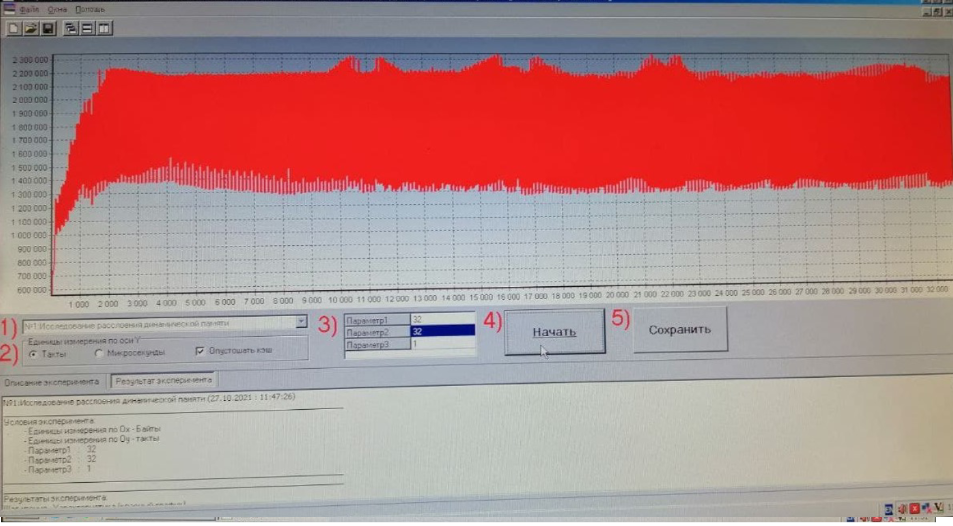
\includegraphics[scale=0.7]{images/experiment_1_2}
		\caption{Эксперимент №1, случай 2}
		\label{img:experiment_1_2}
	}
\end{figure}

На рисунке \ref{img:experiment_1_3} представлен график, полученный в результате эксперимента с исходными параметрами:
\begin{itemize}
	\item максимальное расстояния между	читаемыми блоками (К) = 128;
	\item шаг увеличения расстояния между читаемыми 4-х байтовыми ячейками (Б) = 64;
	\item размер массива (М) = 1.
\end{itemize}

\begin{figure}[H]
	\centering{
		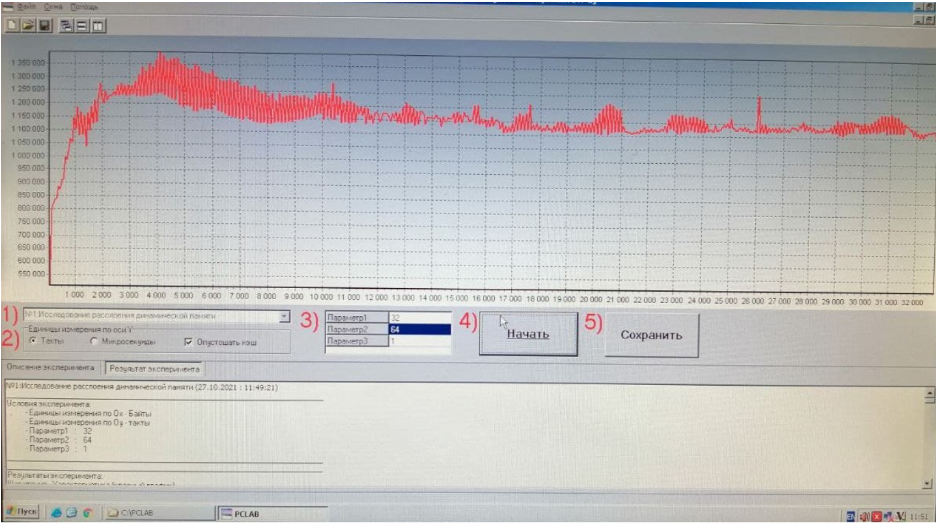
\includegraphics[scale=0.7]{images/experiment_1_3}
		\caption{Эксперимент №1, случай 3}
		\label{img:experiment_1_3}
	}
\end{figure}

Первый пик, который мы видим на рисунке \ref{img:experiment_1_1} -- адресное расстояние между страницей в одном банке и следующей страницей в том же банке. Это адресное расстояние равно 1024.

При просмотре результатов эксперимента № 1 случая 2, где параметр " Шаг увеличения расстояния между читаемыми 4-х байтовыми ячейками" равен 64, можно заметить, что первый запрос на 64б ждет нормальное количество времени, а вот вторые ждут меньше, третьи опять нормальное количество времени и т.д. То есть можно сказать, что размер одной страницы у нас равен 128б, так как когда мы делаем запрос данных с какой-либо страницы, она загружается полностью, и тогда следующий запрос данных к этой странице уже будет длиться меньше по количеству времени. 

Тогда можно сказать, что если "размер страницы" = "размер динамической памяти" / "количество страниц", то имея результаты приведенные выше, количество страниц = $1024 / 128 = 8$.

На современных процессорах невозможно анализировать волну памяти, так как трансляция физических адресов на строки, столбцы и банки DRAM изменилась и держится в секрете.

\subsection*{\textbf{Вывод}}
Оперативная память неоднородна, и для обращения к последовательно расположенными данным может потребоваться различное количество времени. Поэтому, при создании программ необходимо учитывать расслоение памяти при обработке данных.